% !TEX root=/home/tavant/these/manuscript/src/manuscript.tex




\chapter{Polytropic sheath model in the presence of electron emission}
\label{ch-4}

\begin{Chabstract}
  
%e modify the polytropic sheath model with secondary electron emission
We add to the non-isothermal sheath model developed in \cref{ch-3} the secondary electron emission.
using the \ac{PIC} simulations, we observe that the polytropic index is almost constant when varying the cross-over energy $\crover$.
The predictions of the polytropic sheath model are compared to the \ac{PIC} simulations results presented in \cref{ch-2}.
The modified sheath model is included in a \ac{1D} fluid model.
\end{Chabstract}

{\bf IV. Polytrotic sheath model with SEE} 20 pages
\begin{zzz}
  This chapter goes beyond the actual modified sheath model in order to add SEEs.
  This require some time to develop before writting !

  5.1 Kinetic effects of the SEE on the EVDFs  4 pages

  5.2 SEE effects on the Fluid model  5 pages

  5.3 Validation against the Parametric 2D PIC simulation results. 2 pages
  
  5.4 1D fluid model with modified wall model. 4 pages
  
  5.4Bis Global model (Vivien's) with modified wall model. 4 pages
\end{zzz}

\minitoc
% 
% What is complicated here is the definition of the electron temperature, that include both primary and secondary electrons.
% Should we
% \begin{itemize}
%   \item Use a 2 fluid( so 1 electron) with a fluid model that includes the SEE ?
%   \item Use a 3 fluid model, that would  include folly absorbed primary electrons (simply polytropic) and emitted electrons, with strictly positive velocity.
% \end{itemize}
% 
% In the First case, the electron temperature is simple to define.
% But the closure equation may need to be changed.
% 
% the second case is more simpler, mathematicaly.
% 
% References:
% Il y a déjà eu beaucoup de travaux, mais aucun model fluides !
% 
% \citet{meezan2002} : Bolzmann solver, 2-Te EVDF, SEE compared with Maxwellian
% 
% \citet{smirnov2004} : MCC code, 2-Te EVDF. Mais fake EVDI effect via collisions
% 
% \citet{sydorenko2006a} : Beam in EVDF because of 1D PIC-MCC 
% 
% \citet{raitses2006} : "strong anisotropy : facteur 4",  compare Mesures avec fluids codes: says disagriment. Talks about 
% 
% \citet{ahedo2002} : sheath-presheath model with SEE with bolzmann electron, Sagdeev potential, SCL regime avec saturations 
% 
% \citet{ahedo2003} : 1D axial model avec wall interactions (SEE et SCL), plum with section increase (A(z)) 
% 
% \citet{ahedo2005} : Fluid model with SEE, with partial trapping and partial beams
% 
% \citet{raitses2005} : SCL regime and Te saturation (where he says that the SCL may not be responsible ??)
% 
% \citet{barral2003a} : 1D model, anisotrop electrons ({\bf must read to know how}), shows saturation at SCL with large anisotropy

{\bf \Large A lire}

\citet{sydorenko2007} :  non maxwellian EVDF

\citet{raitses2005a} : electron-wall interaction

\citet{jolivet2000} : SEE effect on EVDF 

% !TEX root=/home/tavant/these/manuscript/src/manuscript.tex


\section{Polytropic index in the \ac{HET} \ac{PIC} simulations}
\label{sec-PIC_poly}

\begin{figure}[hbtp]
  \centering
  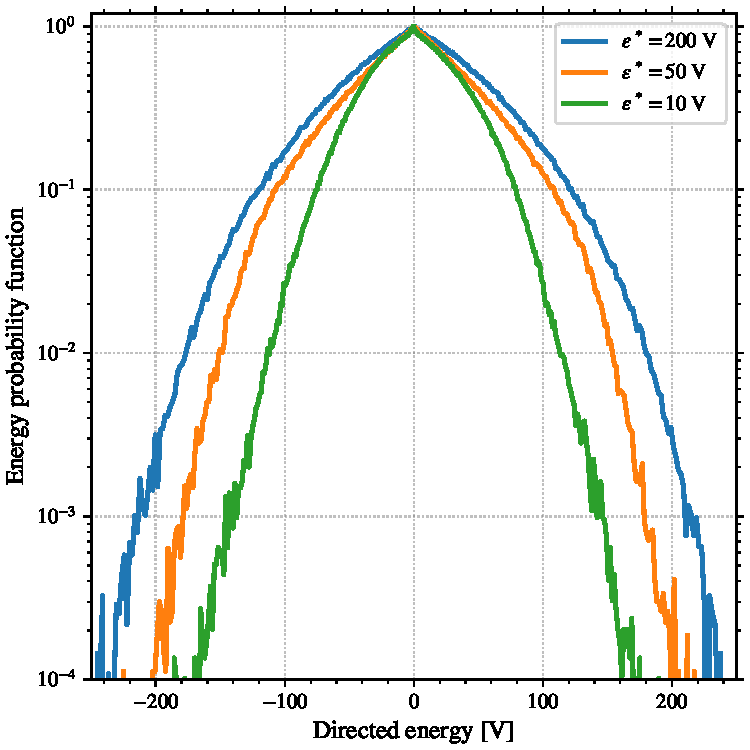
\includegraphics[width=\defaultwidth]{EVDF_Bulk.pdf}
  \caption{Electron velocity distribution function at the center of the simulation, for different values of $\crover$.}
  \label{fig-evdf_epsstar}
\end{figure}

\begin{figure}[hbtp]
  \centering
  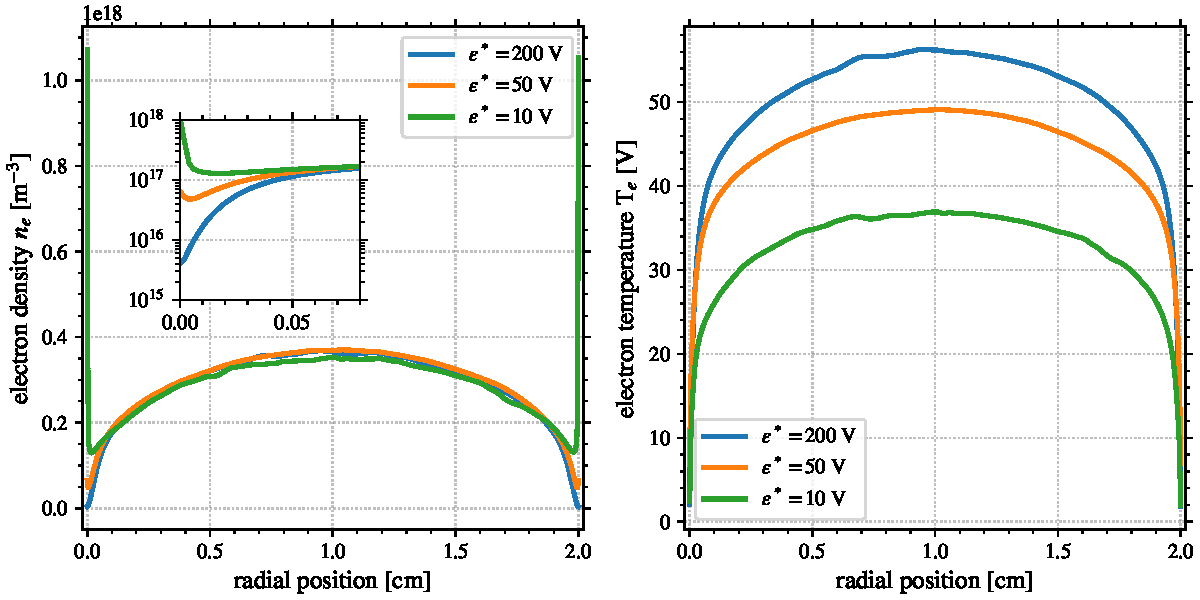
\includegraphics[width=\textwidth]{ne_Te_profiles.pdf}
  \caption{Radial profiles of (left) the electron density and (right) the electron temperature, for different values of $\crover$.}
  \label{fig-radial_profiles_see}
\end{figure}


\begin{figure}[hbtp]
  \centering
  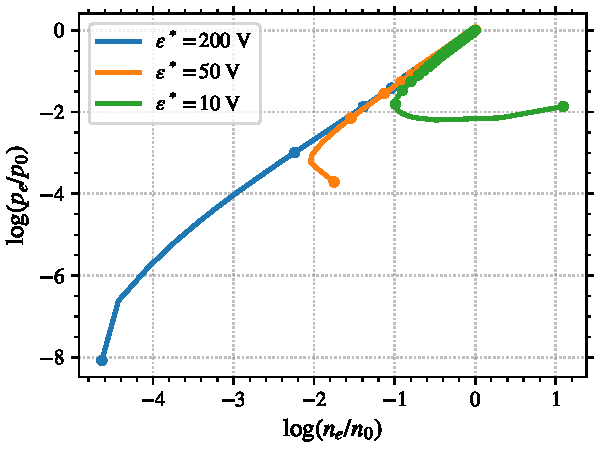
\includegraphics[width=\defaultwidth]{SEE_polytropic_presheath_and_sheath.pdf}
  \caption{electron pressure as a function of the electron density normalized by the center variable, in log scale. Markers are every 10 cells (around 1$\lde$)}
  \label{fig-log_pe-ne}
\end{figure}

\renewcommand\subfigurewidth{3in}

\begin{figure}[hbtp]
  \centering
  \begin{tabular}{c c}
    \subfigure{SEE_polytropic_presheath}{a}{20,20} & 
    \subfigure{SEE_polyfit}{a}{20,20} 
  \end{tabular}
  \caption{Polytropic fit for different values of $\crover$. The sheath (10 cells) are removed from the plots.}
  \label{fig-polyfit_see}
\end{figure}

\FloatBarrier
{\bf Conclusion: $\gamma = 1.35$ in presheath and $\partial{\gamma} / \partial \crover = 0 $}

\paragraph{Hypothesis H1: } Polytropic model until the wall and $\gamma = 1.35$ (might be explained by \cref{{fig-evdf_epsstar}}, and by the fact that we care only on the forward temperature, so not distorted by the secondary electrons).

\paragraph{Hypothesis H2: } From {\bf H1}, and with the 2-$\Te$ hypothesis, we have $\rate = \rate_{\rm Maxw}(\Tew)$, were $\Tew$ can be computed from $Teb$, $\gamma$ and $\dphi$.

\paragraph{Hypothesis H3: } Current equality at the wall : $\Gamma_i + \rate \Gamma_e = \Gamma_e$. This is not a surprising hypothesis.

\section{Sheath model with polytropic electron and SEE}

With {\bf H1, H2} and {\bf H3} we have, as developed in \cref{sec-fluidPIC} with \cref{eq-gi,eq-ge,eq-tew}:
\begin{equation}\label{eq-sheathsee}
  (1 - \rate_{\rm Maxw}(\Tew) )\left[ 1 +\frac{\gamma -1}{\gamma} \frac{ \dphi_0}{ \Te_0}  \right]^{\frac{1}{\gamma - 1}} \sqrt{1 - \frac{\gamma -1}{\gamma}\frac{\dphi_0}{\Te_0}} = \sqrt{\frac{4 \gamma \pi m_e}{m_i}}
\end{equation}
In contrast with \cref{eq-sheath}, now the sheath potential $\Delta \phi$ depends on $\rate$ with depends on $\Te$.
Hence, $\dphi$ is not fully normalized.

\begin{figure}[hbtp]
  \centering
  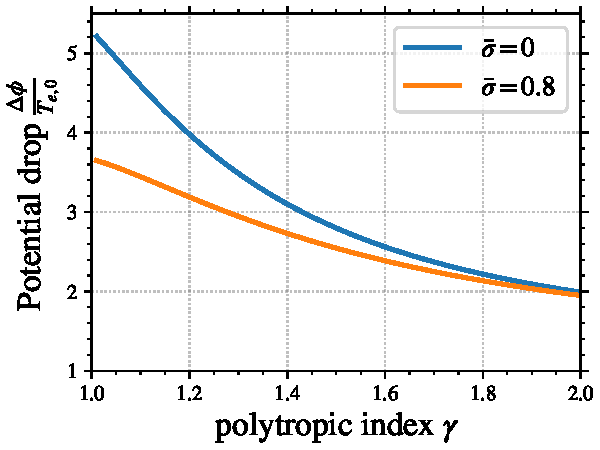
\includegraphics[width=\defaultwidth]{Sheath_drop_with_SEE.pdf}
  \caption{Potential drop $\dphi$ normilized by the bulk electron temperature $\Te_0$ as a function of the polytropic index $\gamma$ for a xenon plasma ($m_i = 131\,\dalton$). The emission rate $\rate$ is fixed for clarity.}
  \label{fig-dphi_see}
\end{figure}

\begin{figure}[hbtp]
  \centering
  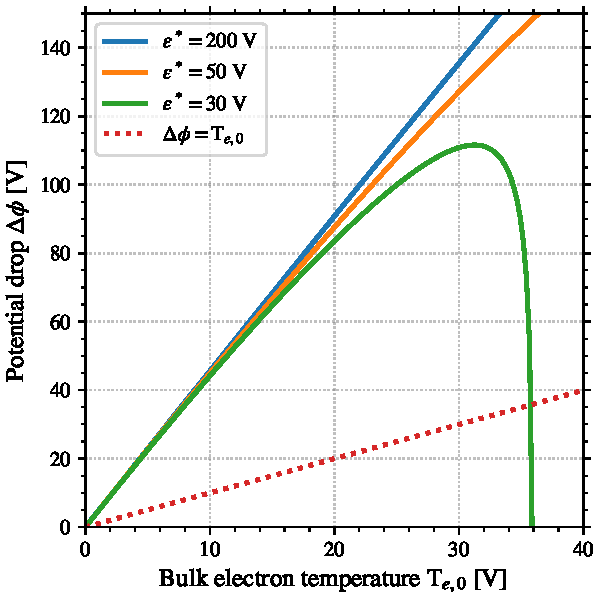
\includegraphics[width=\defaultwidth]{RSO_criteria_polytropic.pdf}
  \caption{ Plasma potential drop to the wall as a function of the electron temperature for different values of the cross-over energy $\crover$ using \cref{eq-sheathsee,eq-seemaxw}. The dashed line is $\dphi=\Te$. Similar to  \cref{fig-dphivsTe} but with polytropic electron of index $\gamma=1.35$}
  \label{fig-rso_crit_see}
\end{figure}

\FloatBarrier

\section{Comparison with PIC simulations} \label{subsec-picandmodel}

\begin{figure}[hbtp]
  \centering
  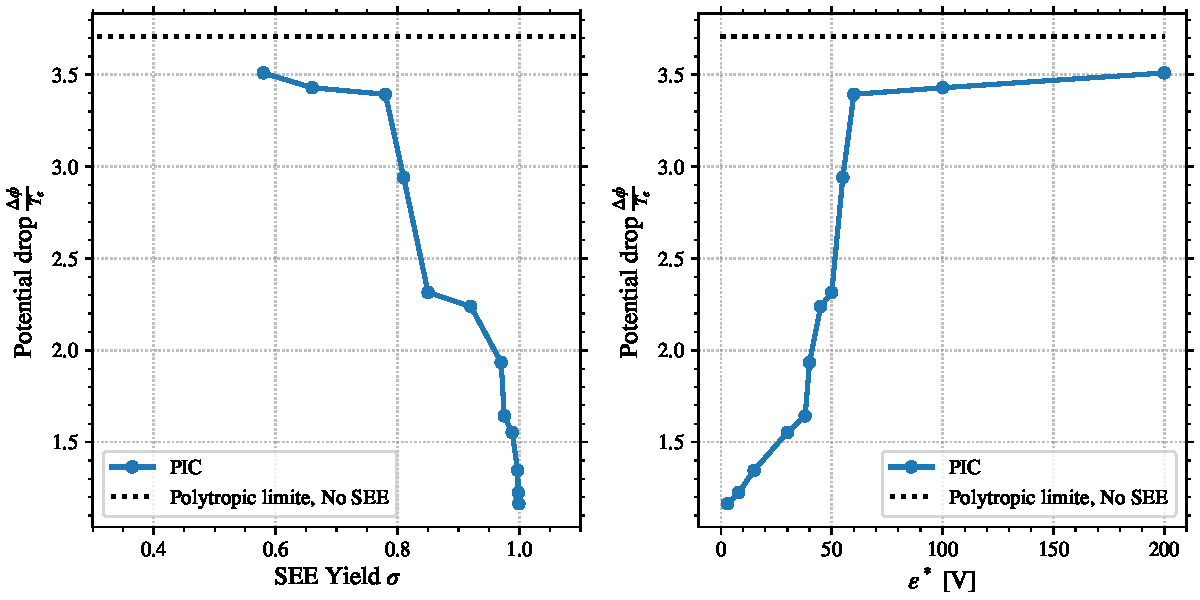
\includegraphics[width=\textwidth]{dphi_polytropic_noSEE}
  \caption{PIC simulation results (with SEE) compared to the polytropic limit without SEE.}
  \label{fig-polytropic_pic_noSEE}
\end{figure}

\begin{figure}[hbtp]
  \centering
  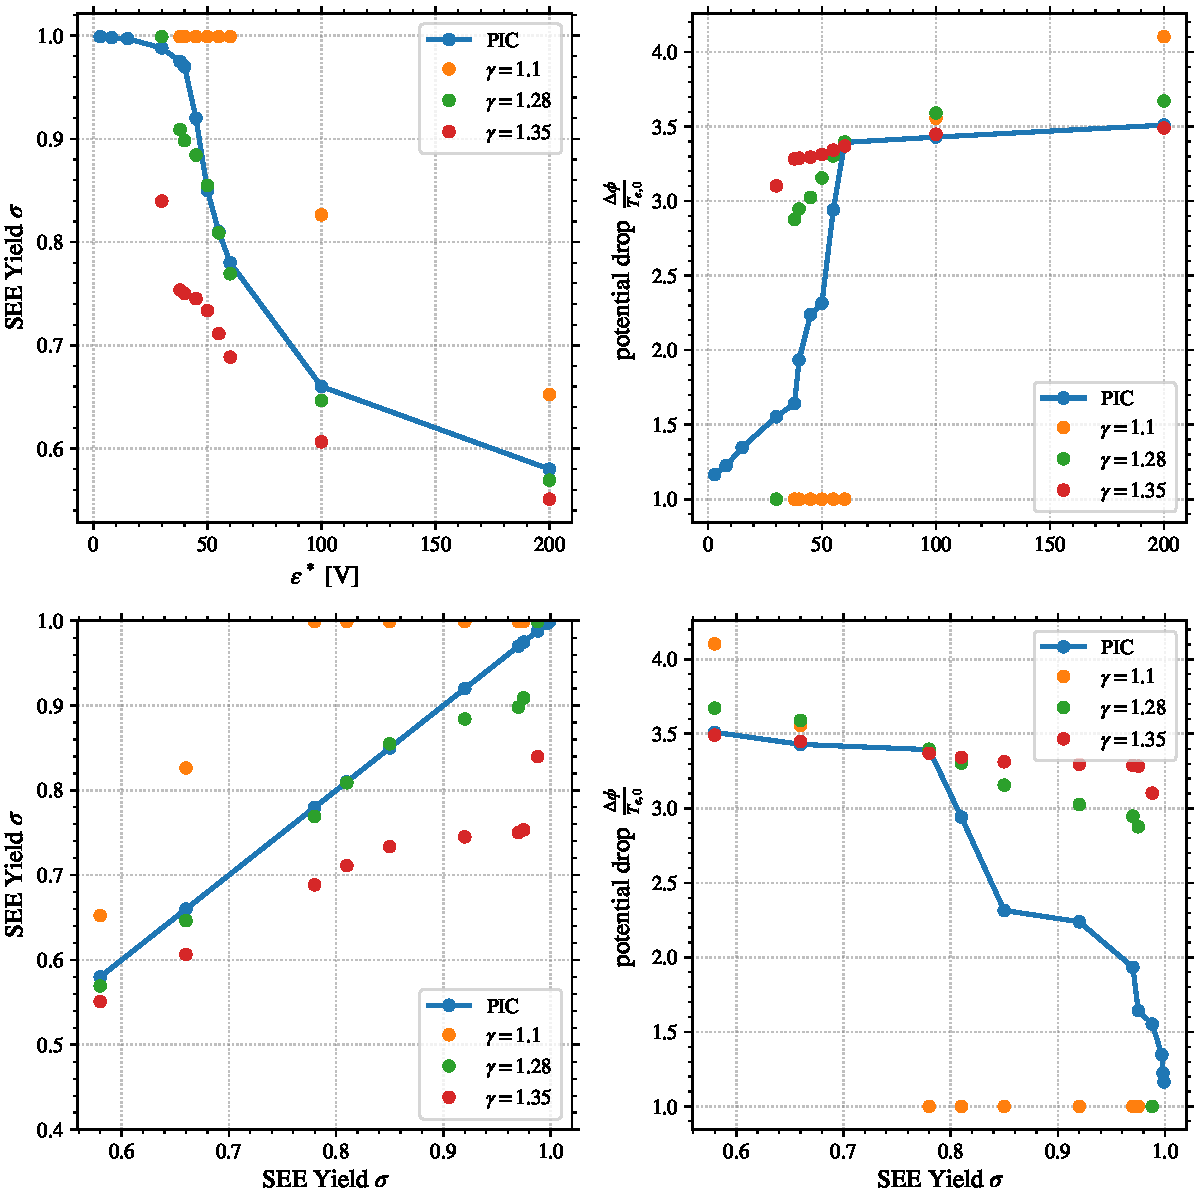
\includegraphics[width=\textwidth]{Summary_polytropic_SEE.pdf}
  \caption{Comparison of the PIC simulation results with the polytropic model with SEE.}
  \label{fig-polytropic_see_summary}
\end{figure}



% !TEX root=/home/tavant/these/manuscript/src/manuscript.tex

% \FloatBarrier
\section{Sheath model with polytropic electrons and electron emission}
\label{sec-fluid_poly_see}

\let\oldrightmark=\rightmark
\renewcommand\rightmark{\expandafter\MakeUppercase{Sheath with polytropic electron and SEE}}


\subsection{Definition of the sheath equation} \label{subsec-def_sheat_see}

We have seen in \cref{sec-PIC_poly} that even in the presence of electron emission from the wall, the electrons can be described using a polytropic state law.
The value of the polytropic index obtained from the mean electron density and temperature is for $\crover \geq 40 \,\volt$ is $\gamma = 1.36$.
% Using the electron distribution function, the evolution of the forward electron seems to follow a polytropic low of index $\gamma=1.28$.
Hence, we modify the polytropic sheath model of \cref{sec-fluid} to take into account the electron emission from the wall.
This modifies the current equality at the wall to
\begin{equation} \label{eq-see-J_eq}
  \Gamma_i = (1 - \rate) \Gamma_e.
\end{equation}

\paragraph{Sheath model with constant emission rate\\}

Using \cref{eq-gi,eq-ge,eq-tew} for $\Gamma_i$ and $\Gamma_e$, we obtain the equality
\begin{equation}\label{eq-sheathsee}
  (1 - \rate )\left[ 1 +\frac{\gamma -1}{\gamma} \frac{ \dphi_0}{ \Te_0}  \right]^{\frac{1}{\gamma - 1}} \sqrt{1 - \frac{\gamma -1}{\gamma}\frac{\dphi_0}{\Te_0}} = \sqrt{\frac{4 \gamma \pi m_e}{m_i}}
\end{equation}

Similarly to the case without electron emission in \cref{sec-fluid}, \cref{eq-sheathsee} cannot be solved analytically, but it can be solved numerically.
The solution for $\rate=0.8$ is compared to the case without electron emission ($\rate=0$) for a \ac{Xe} plasma in \cref{fig-dphi_see}.
As expected, the potential difference decreases with increasing $\rate$.
We see that the gap between the two cases decreases when $\gamma$ increases from 1 to 2.

\begin{figure}[!hbt]
  \centering
  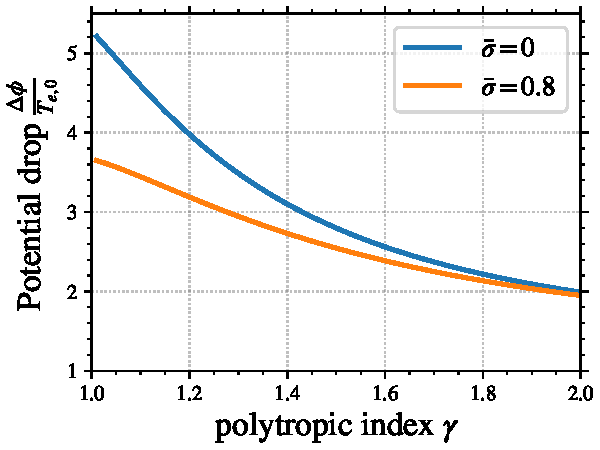
\includegraphics[width=\defaultwidth]{Sheath_drop_with_SEE.pdf}
  \caption{Potential drop $\dphi$ normalized by the bulk electron temperature $\Te_0$ as a function of the polytropic index $\gamma$ for a xenon plasma ($m_i = 131\,\atomicmass$). The emission rate $\rate$ is fixed either at $\rate=0$ or $\rate=0.8$.}
  \label{fig-dphi_see}
\end{figure}

\paragraph{Sheath model with varying emission rate\\}

In fact the electron emission rate is a function of the electron temperature at the wall.
Using the same hypothesis as in \cref{eq-ge} (mostly a Maxwellian \ac{EVDF} at the wall), we define the emission rate from \cref{eq-seemaxw} by
\begin{equation} \label{eq-seemaxw_poly}
  \rate = 
  \begin{cases}
    \ratemaxw(\Tew) =  \sigo + ( 1 - \sigo) \frac{ 2 \Tew  }{\crover} \\
    \ratecr \text{ \quad, if } \ratemaxw(\Tew) > \ratecr
  \end{cases}
\end{equation}
with $\ratecr = 0.983$ corresponding to the \ac{SCL} regime, and the electron temperature at the wall
\begin{equation} \label{eq-Tewall}
  \Tew = \Teb - \frac{\gamma - 1}{\gamma } \dphi.
\end{equation}


Noting $\chi = \frac{\gamma -1}{\gamma} \frac{ \dphi_0}{ \Teb} $, we finely obtain the sheath equation to be solved
\begin{equation} \label{eq-costseepoly}
  f(\chi) = \left[ 1 + \chi  \right]^{\frac{1}{\gamma - 1}} \sqrt{1 - \chi} - \frac{  \sqrt{4 \gamma m_e / m_i}}{1 - \rate (\Teb, \chi )} = 0.
\end{equation}

\Cref{eq-costseepoly} depends now explicitly on $\Teb$ though $\rate$.
Hence, the solution of $f(\chi)=0$ is no longer independent of $\Teb$, which adds a free parameter when solving the sheath equation.
\Cref{fig-costfunction} shows the evolution of $f(\chi)$ of \cref{eq-costseepoly} for $\gamma = 1.36$, $\Teb=40\,\volt$ and $\crover=50\,\volt$.

\begin{figure}[!hbt]
  \centering
  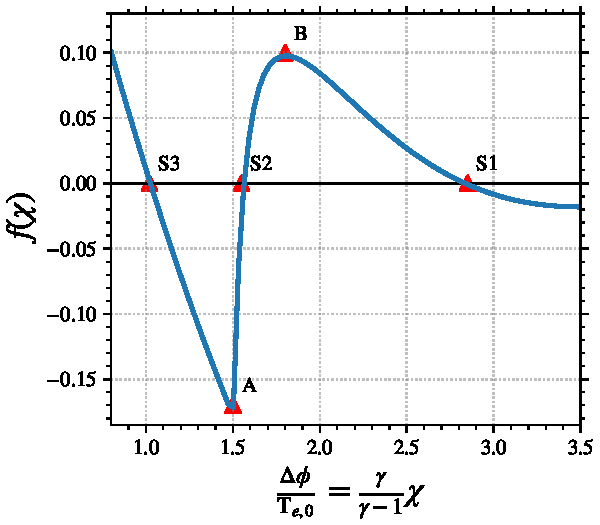
\includegraphics[width=\defaultwidth]{cost_function_solo}
  \caption{Value of $f(\chi)$ of \cref{eq-costseepoly} for $\gamma = 1.36$, $\Teb=40\,\volt$ and $\crover=50\,\volt$. The five red triangular markers represents five points of interest\string: the three markers S1, S2, and S3 are solutions of $f(\chi) = 0$; and the markers A and B are two local extrema. }
  \label{fig-costfunction}
\end{figure}

We see that $f(\chi)$ of \cref{eq-costseepoly} is rather complex.
Five points of interest are marked and labeled in \cref{fig-costfunction} to ease the reading\string: 
\begin{enumerate}
  \item S1, S2, and S3 represents the points at which $f(\chi)=0$, i.e. the solutions of  \cref{eq-costseepoly}
  \item A and B are two local extrema.
\end{enumerate}

The courbe $f(\chi)$ is composed of two continuous branches that join at the point A in \cref{fig-costfunction}.
The two branches corresponds to the two cases of \cref{eq-seemaxw_poly}. Hence, the point A corresponds to the value of $\dphi/\Teb$ for which  \[ \sigo + ( 1 - \sigo) \frac{ 2 \Tew  }{\crover} = \ratecr = 0.983. \]

The branch at the left of A corresponds to the \ac{SCL} regime, and has one solution S3 to $f(\chi)=0$ at $\dphi / \Teb \simeq 1$.
This solutions is the same as in the isothermal case \citep{hobbs1967}.
The branch at the right of A passes by a local maximum B and presents two roots S1 and S3.

The existence of the three solutions depends on the values of $\crover$, $\Teb$ and $\gamma$.
\Cref{fig-costfunction_multiple} shows the impact of the evolution of $\Teb$ and $\crover$, with $\gamma$ constant.
We can see that when $\Teb$ decreases, or $\crover$ increases, the points A and B move upward.
Consequently, for low values of $\Teb$ (respectively large values of $\crover$) the point A can be above the line $f(\chi) = 0$, hence  \cref{eq-costseepoly} presents only the root S1.
In contrast for high values of $\Teb$ (respectively low values of $\crover$) the point B is below $f(\chi) = 0$, so that only S3 is solution of  \cref{eq-costseepoly}.
For intermediate values of $\Teb$ and $\crover$, A and B are located on both sides of $f(\chi) = 0$, so that the three roots S1, S2, and S3 exist.
\renewcommand\subfigurewidth{0.47\textwidth}

\begin{figure}[!hbt]
  \centering
  \begin{tabular}{@{} c c}
    \subfigure{cost_function_bis.pdf}{a}{25,25} &
    \subfigure{cost_function_2bis.pdf}{b}{25,25} \\
  \end{tabular}
  \caption{Value of $f(\chi)$ of \cref{eq-costseepoly} for $\gamma = 1.36$ and different values of $\Teb$ and $\crover$. ({\bf a}) shows the impact of the evolution of $\Teb$ with $\crover=50\,\volt$, and ({\bf b}) shows the impact of the evolution of $\crover$ with $\Teb=35\,\volt$. }
  \label{fig-costfunction_multiple}
\end{figure}

\Cref{fig-schematic-solutions} illustrates the three coexisting sheath solutions.
The red solid line  with the largest potential drop to the wall represents the solution S1, which is the standard sheath.
This solutions leads to the largest electron temperature drop to the wall, hence the smallest \ac{SEE} rate.
The dashed blue line, with a potential well close to the wall, corresponds to the root S3 in the \acs{SCL} regime, for which $\rate=\ratecr$ and with $\dphi \simeq \Teb$.
Lastly, the dash-dotted green line represents S2 the intermediate solution.
 
\begin{figure}[hbtp]
  \centering
  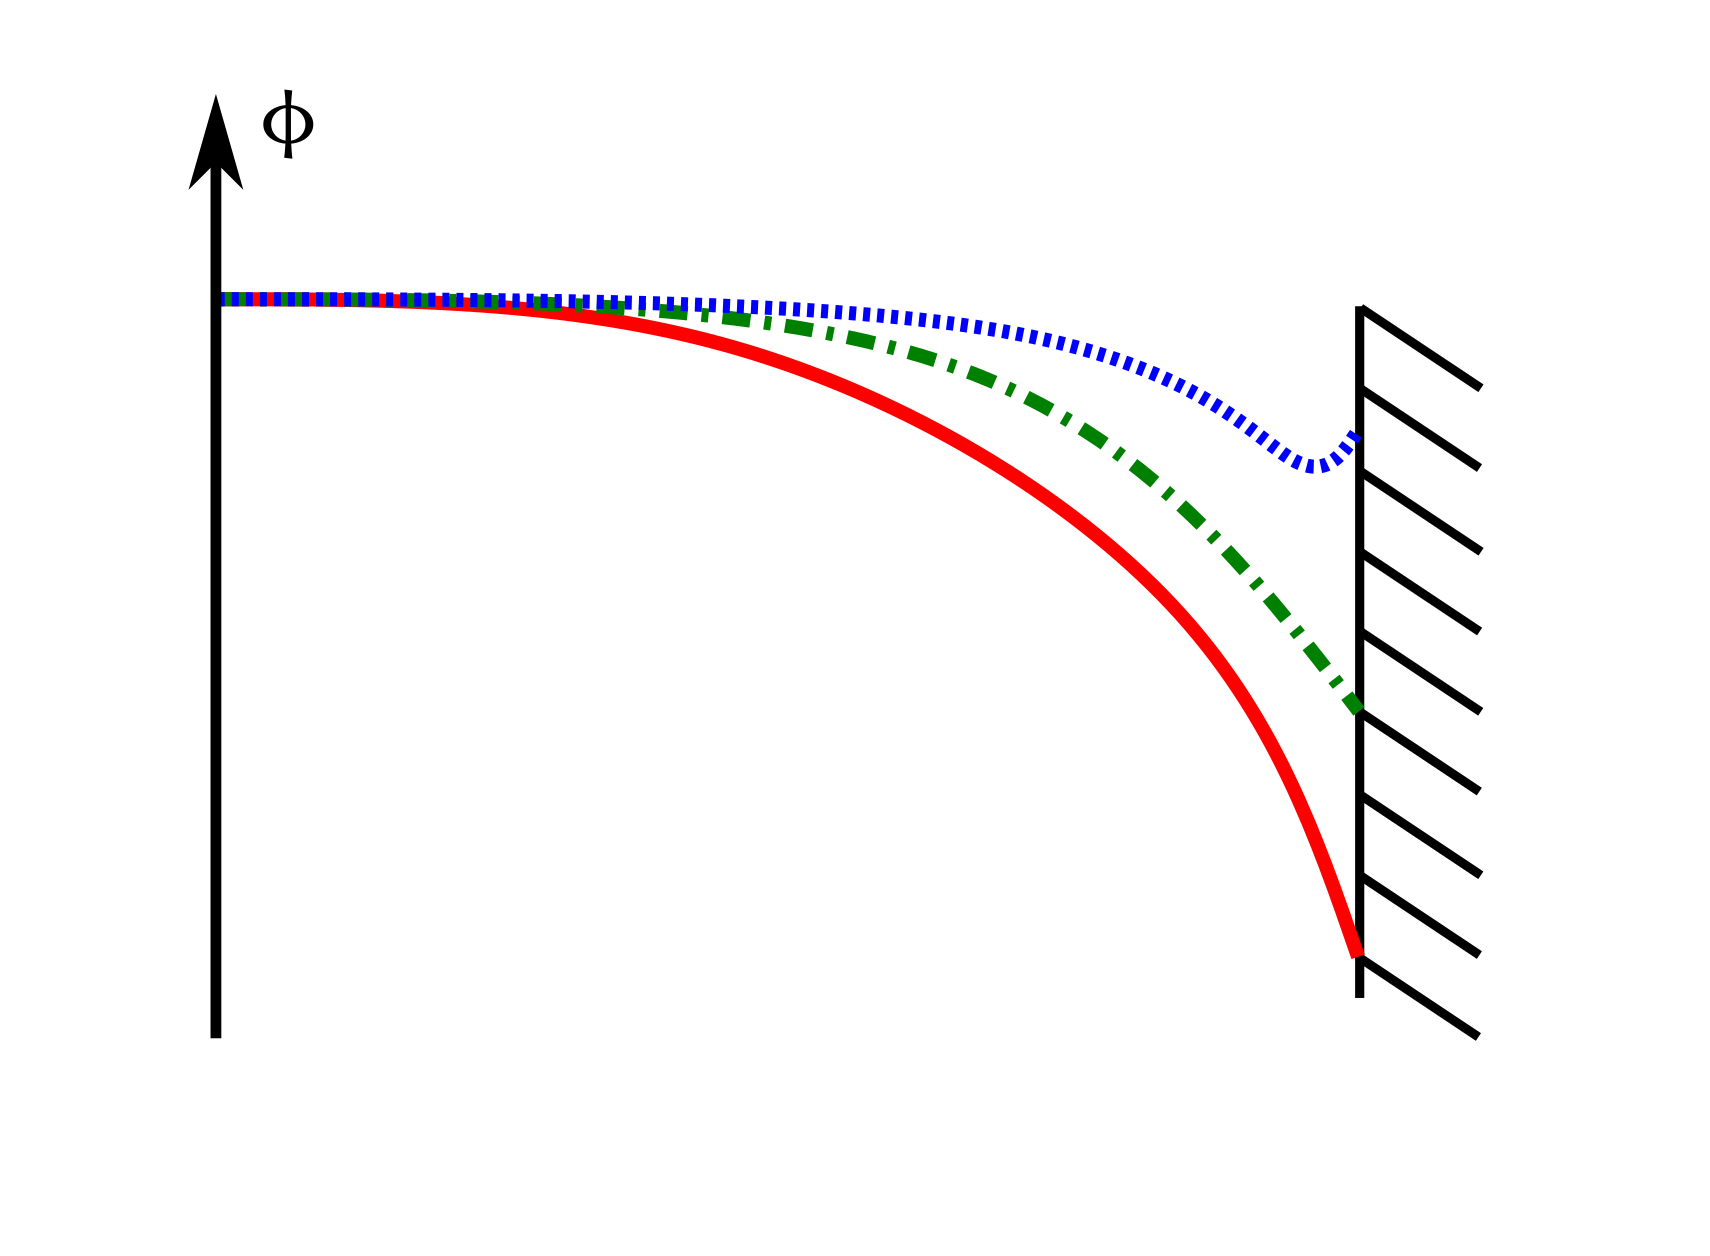
\includegraphics[width=\defaultwidth]{sheath_solutions.png}
  \caption{Schematic representation of the plasma potential profile in the sheath to the wall for the three coexisting solutions. The red solid line is the standard solution, with the lowest \acs{SEE} rate; the dashed blue line corresponds to the \acs{SCL} regime, with $\rate=\ratecr$; the dash-dotted green line is the intermediate solution, with an intermediate \acs{SEE} rate.  }
  \label{fig-schematic-solutions}
\end{figure}



\Cref{fig-iso_poly} shows the evolution of the sheath potential drop and the \ac{SEE} rate as a function of $\Teb$ for the case $\crover=50\,\volt$.
Both the isothermal sheath and the polytropic model using $\gamma=1.36$ are showed. 
The result of the isothermal sheath model was previously shown in \cref{fig-dphivsTe}  in \cref{ch-2}.
For the solution of the polytropic sheath model, the branches corresponding to the three solutions S1, S2, and S3 are labeled.
The light green area highlights the temperature range with the three coexisting solutions.
The lower bounds of the area is noted $\Te^2$ and the upper bound is noted $\Te^1$
\renewcommand\subfigurewidth{0.65\textwidth}

\begin{figure}[!hbt]
  \centering
  \begin{tabular}{@{} c}
    \subfigure{Iso_vs_poly_dphibis}{a}{25,18} \\
    \subfigure{Iso_vs_poly_rate}{b}{20,18} 
  \end{tabular}
  \caption{Evolution as a function of the electron temperature $\Te$ for $\crover=50\,\volt$ of ({\bf a}) the plasma potential drop to the wall $\dphi$, and ({\bf b}) the SEE rate $\ratemaxw$ using the polytropic sheath model ($\gamma = 1.36$) and the isothermal sheath model. The labels S1, S2 and SCL regime correspond to the three solutions illustrated in \cref{fig-schematic-solutions}. The light green area highlights the temperature range with three solutions.}
  \label{fig-iso_poly}
\end{figure}

\renewcommand\subfigurewidth{0.47\textwidth}

We see in \cref{fig-iso_poly}.{\bf a} that $\dphi$ is significantly impacted by the polytropic law.
In particular the maximum potential drop which is more than twice as high as the isothermal maximum.
In addition, we see in \cref{fig-iso_poly}.{\bf b} that the polytropic sheath model predicts a \ac{SEE} rate smaller than the isothermal model.
This is due to the fact that the polytropic state law reduces the electron temperature at the wall, hence decreases the electron emission rate for a given $\Teb$.
Consequently, the electron bulk temperature can access higher temperature, compared to the one observed in \cref{fig-dphivsTe}.


\subsection{Theoretical values of the critical electron temperatures} \label{subsec-theo_Tecr}

  As shown in \cref{fig-costfunction}, for a given $\Teb$ $f(\chi)$ defined by  \cref{eq-costseepoly} presents a local minimum and a local maximum, labeled A and B respectively in \cref{fig-costfunction}.
  Therefore, there exist two values of $\Teb$ for which either the minimum or the maximum of the $f(\chi)$ crosses exactly the horizontal axis.
  These values, noted $\Te^1$ and $\Te^2$ corresponds respectively to the upper and lower bounds of the electron temperature range over which the three solutions coexist.
  These threshold temperatures can be seen for $\gamma=1.36$ in \cref{fig-iso_poly}, where $\Te^1\simeq 55\,\volt$ and $\Te^2\simeq 35\,\volt$ 

  \paragraph{Maximum electron temperature value for regime {\bf III}, $\Te^1$\\}

    The first critical electron temperature  $\Te^1$  corresponds to the maximum temperature of the root S1, which is the usual monotonic sheath (corresponding to regime {\bf III}).
    It is defined as the temperature for which the the local maximum B crosses the line $f(\chi)=0$.
    As it is a double solution, it corresponds to the solution of \cref{eq-costseepoly} that is also a solution of its derivative with respect to $\chi$\string:
    \[ \deriv{f(\chi)}{\chi} = 0. \]
    Once again, the equation is not trivial, and cannot be solved analytically, thus we solve it numerically.

    \begin{figure}[hbt]
      \centering
      \begin{tabular}{@{} cc}
        \subfigure{Maximum_Te1_epsilon.pdf}{a}{20,20} &
        \subfigure{Maximum_Te1_gamma.pdf}{b}{20,15} \\
      \end{tabular}
      \caption{Variation of $\Te^1$  ({\bf a})  as a function of $\crover$ for two values of $\gamma$, and ({\bf b})  as a function of $\gamma$ for two values of $\crover$.}
      \label{fig-Te1_epsi}
    \end{figure}

    \Cref{fig-Te1_epsi} shows the variation of $\Te^1$ as a function of   $\crover$  and $\gamma$.
    We see that the maximum temperature $\Te^1$ increases linearly with $\crover$.
    This was expected, as in \cref{eq-costseepoly}, the only time that $\Teb$ is explicitly present is in the term $\frac{\Teb}{\crover}$.
    On the other hand, the variation with $\gamma$ follows a power law, monotonically increasing from $30\,\volt$ for $\gamma=1.2$ to $50\,\volt$ for $\gamma=1.4$ in the case $\crover=45\,volt$.

  \paragraph{Minimum electron temperature value for regime {\bf I}, $\Te^2$\\}

    The minimum electron temperature value for regime {\bf I}, $\Te^2$, corresponds to the case where the electron temperature at the wall induces exactly an emission rate $\ratemaxw (\Tew) = \ratecr$.
    Noting $C_1 = \frac{\ratecr - \sigo}{1-\sigo} = 0.964$, we obtain
    \begin{equation} \label{eq-Te2}
      (1-\ratecr) \lp 2 - \frac{C_1 \crover}{2 \Te^2} \rp^{\frac{1}{(\gamma-1)}} \sqrt{\frac{C_1 \crover}{2 \Te^2}} = \sqrt{\frac{4 \gamma \pi m_e}{m_i}}
    \end{equation}

    \Cref{eq-Te2} is solved numerically.
    The solutions for different values of $\crover$ and $\gamma$ are shown in \cref{fig-Te2_epsi}.
    As for $\Te^1$, $\Te^2$ increases linearly with $\crover$.
    It also increases slowly with $\gamma$, from $26\,\volt$ for $\gamma=1.2$ to $30\,\volt$ for $\gamma=1.4$ in the case $\crover=45\,volt$.
    We note that $\Te^2$ increasing more slowly with $\gamma$ compared to $\Te^1$, hence the range of temperature with the three coexisting solutions widen  when $\gamma$ increases.

    \begin{figure}[hbt]
      \centering
      \begin{tabular}{@{} cc}
        \subfigure{Maximum_Te2_epsilon.pdf}{a}{20,25} &
        \subfigure{Maximum_Te2_gamma.pdf}{b}{20,20} \\
      \end{tabular}
      \caption{Variation of $\Te^2$  ({\bf a}) as a function of $\crover$ for two values of $\gamma$, and ({\bf b}) as a function of $\gamma$ for two values of $\crover$.}
      \label{fig-Te2_epsi}
    \end{figure}

% 
% \subsection{Resolution of the sheath equation} \label{subsec-sol_sheat_see}
% \inlinenote{should I keep this section ?}
% 
% \Cref{fig-rso_crit_see} shows the evolution of the sheath potential drop with the electron temperature for different values of $\crover$.
% It is similar to \cref{fig-dphivsTe} but with the use of a polytropic state law for the electrons.
% Two main aspects differ compared to the isothermal model\string: the multiple solutions and the maximal electron temperature of the first solution.
% 
% \begin{figure}[hbt]
%   \centering
%   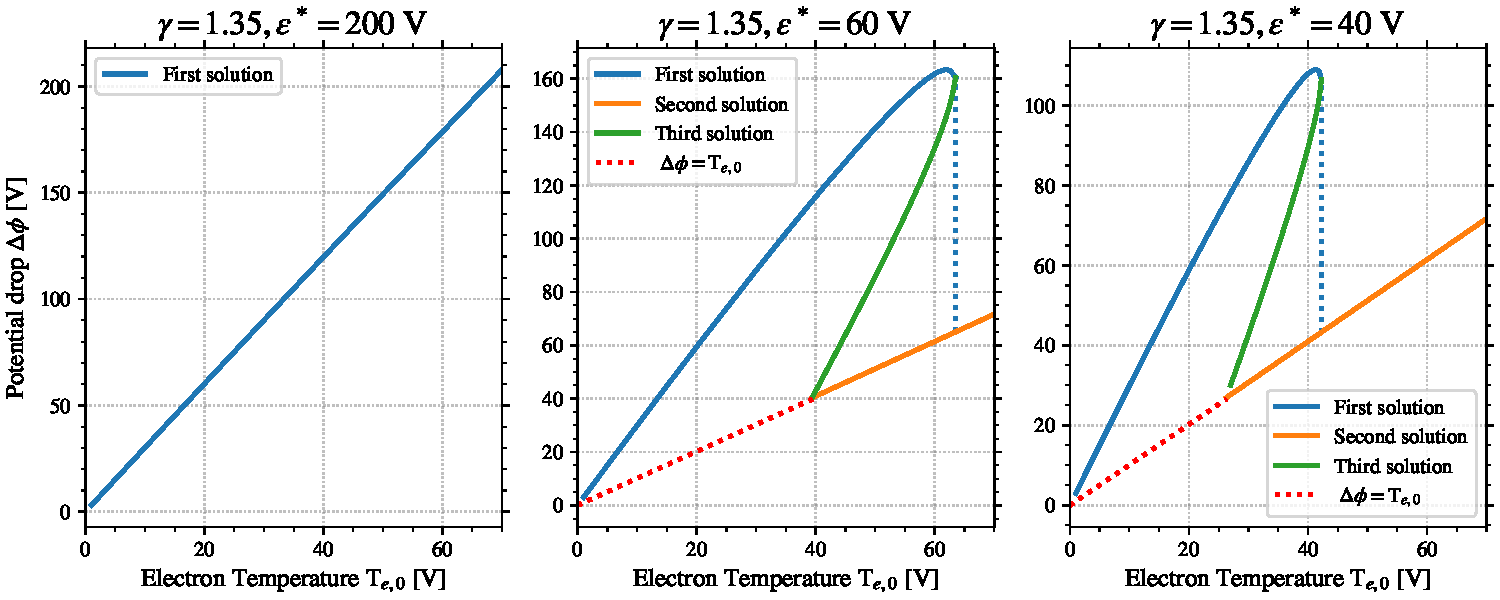
\includegraphics[width=\textwidth]{Potential_drop_poly_see.pdf}
%   \caption{ Plasma potential drop to the wall as a function of the electron temperature for different values of the cross-over energy $\crover$ using \cref{eq-costseepoly}. It is the same results as  \cref{fig-dphivsTe} but with polytropic electron of index $\gamma=1.35$.}
%   \label{fig-rso_crit_see}
% \end{figure}
% 
% We observe in \cref{fig-rso_crit_see} that the electron temperature in the center $\Teb$ can be much higher before the inversion of the plasma sheath potential, compared to \cref{fig-dphivsTe}.


% In addition, for some values of electron temperature, there are three solutions.
% This could explain the oscillations observed in regime {\bf II}.
% Indeed, when the electron temperature increases, the sheath follows the first solutions.
% When the critical electron temperature is reached, the sheath jumps to the third solution.
% It corresponds to the \ac{SCL} regime with an inverted sheath.
% There, the electron temperature in the bulk decreases because of the increased electron power losses at the wall.
% The electron temperature decreases until the second critical temperature, which corresponds to the moment when the third solution disappear, so that the sheath jumps back to the first solution.
% We do not expect the third solution in-between to be observed in the simulations.

% 
% 
% \vspace{1em}
% To summarize, the polytropic law is combined with electron emission to model the sheath.
% The model obtained is richer than the usual isothermal model, as it allows multiple values of potential drop to the wall for the same electron bulk temperature.
% This model only uses the electron bulk temperature and self-consistently computes both the potential drop and the electron emission rate.
% It is compared in the next section to the \ac{PIC} simulation results.


\let\rightmark=\oldrightmark

% !TEX root=/home/tavant/these/manuscript/src/manuscript.tex

% \FloatBarrier

\section{Comparison of the sheath model with PIC simulations} \label{subsec-picandmodel}

  % \begin{figure}[hbtp]
  %   \centering
  %   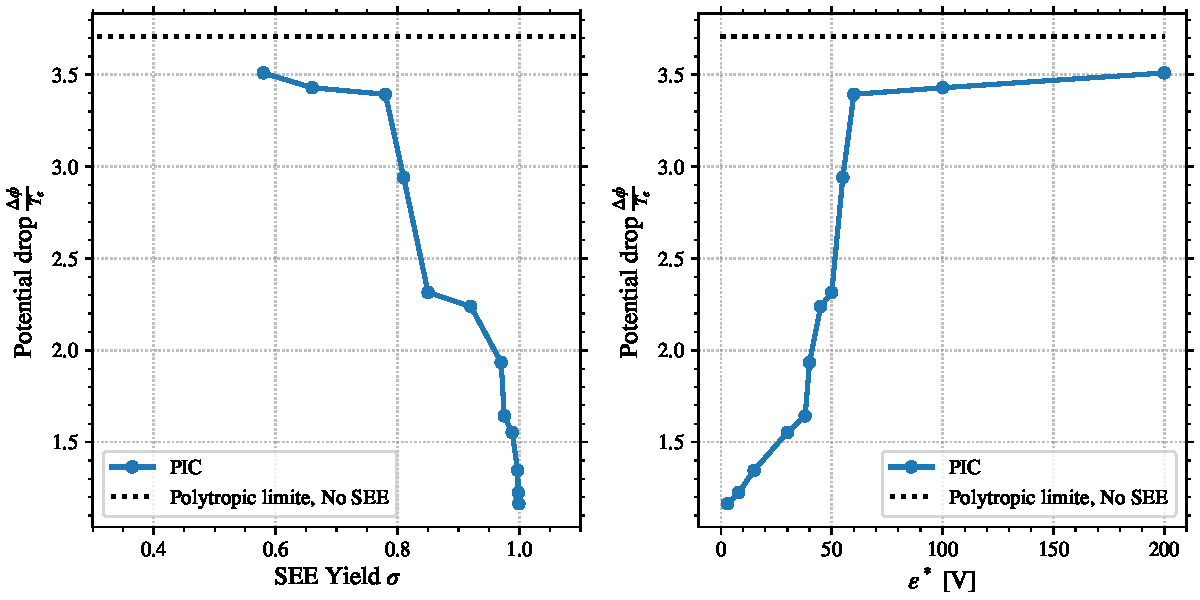
\includegraphics[width=\textwidth]{dphi_polytropic_noSEE}
  %   \caption{PIC simulation results (with SEE) compared to the polytropic limit without SEE.}
  %   \label{fig-polytropic_pic_noSEE}
  % \end{figure}
  % 
  % \begin{figure}[hbtp]
  %   \centering
  %   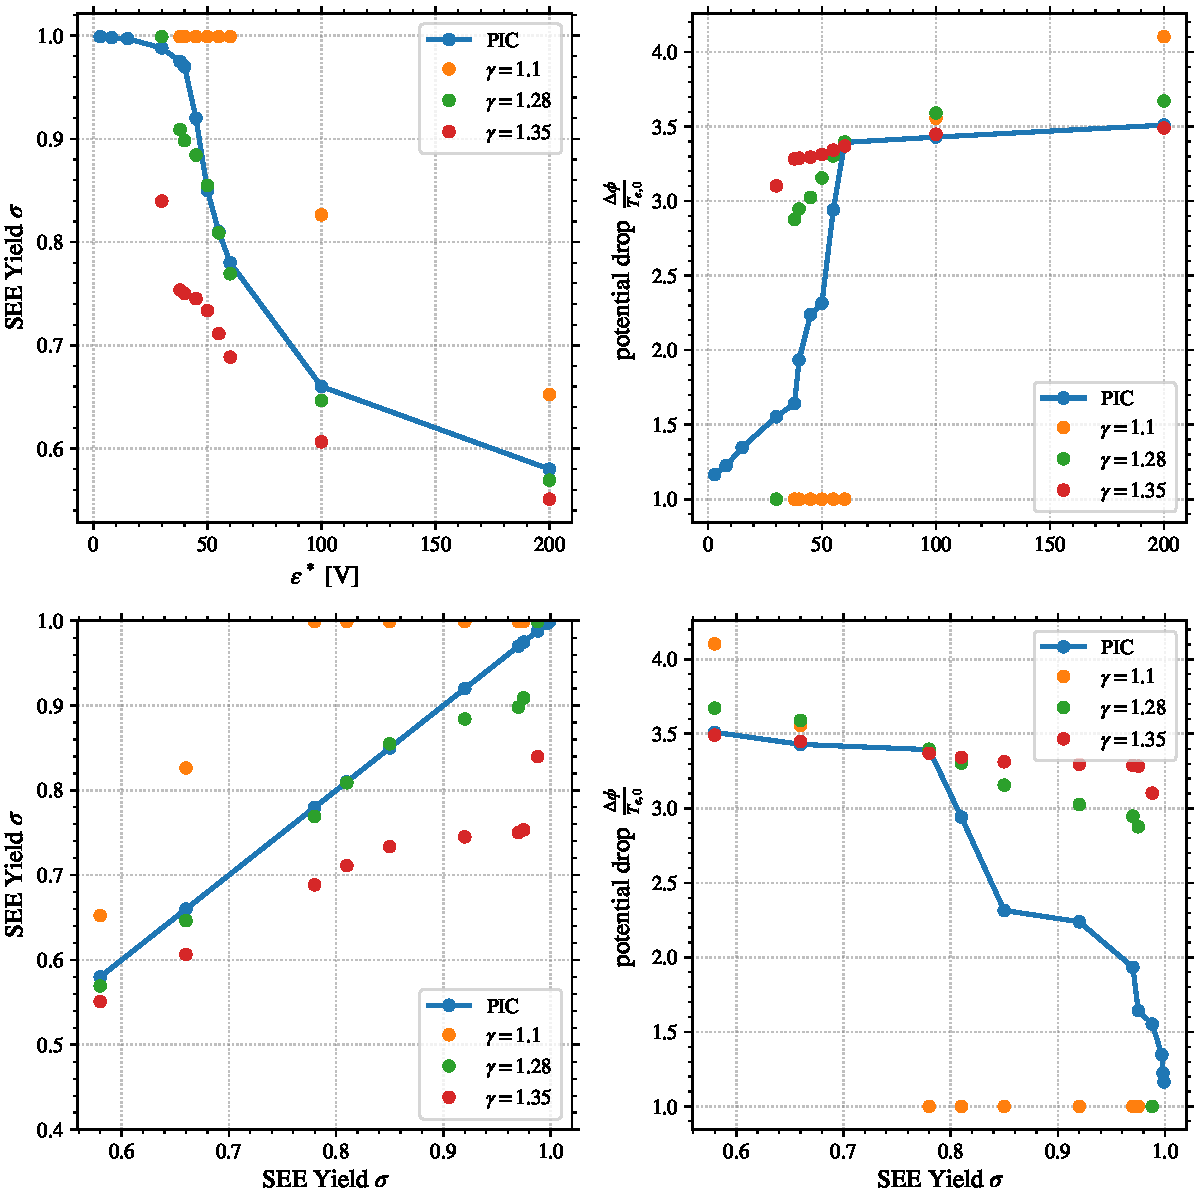
\includegraphics[width=\textwidth]{Summary_polytropic_SEE.pdf}
  %   \caption{Comparison of the PIC simulation results with the polytropic model with SEE.}
  %   \label{fig-polytropic_see_summary}
  % \end{figure}

  We compare in this section the characteristics of the plasma wall interaction observed in the \ac{PIC} simulations with the fluid model developed in \cref{sec-fluid_poly_see}.
  We first compare the mean values using in the parametric study over the crossover energy $\crover$, then we investigate the oscillations of regime {\bf II}.

  \subsection{Parametric study of the modified sheath model} \label{subsec-param_sheath_see}

    The variables of interest to characterize the plasma-wall interaction are the averaged electron emission rate $\rate$ and the plasma potential drop to the wall.
    The only input of the modified sheath model is the electron mean temperature in the bulk $\Teb$, as well as the polytropic index $\gamma$.
    As seen in \cref{sec-PIC_poly}, the polytropic index of the electron population is measured in the \ac{PIC} simulations to be $\gamma=1.35$.
    However, the electrons going toward the wall present a different index, measured from the bulk \ac{EVDF} to $\gamma=1.28$.
    These two values will be compared.

    Using the mean electron temperature measured in the \ac{PIC} simulations, we first compute the plasma potential drop $\dphi$ by solving \cref{eq-costseepoly} with $\gamma=1.35$.
    As shown in \cref{fig-rso_crit_see}, up to three solutions are possible.
    The emission rate $\rate$ is then computed using \cref{eq-seemaxw_Tew}, using the two values for $\gamma$.
    As discussed previously, the rate is limited to $\ratecr=0.982$ to take into account the \ac{SCL} regime.

    The results are shown in \Cref{fig-Poly_model_vs_pic}.
    The plasma potential drop computed is increased by $\Teb/2$ corresponding to the pre-sheath drop to better match the plasma potential measured in the simulations.
    \improvement{The Bhom criterion is slightly modified with the polytropic model, so it should not exactly be $\Teb/2$. however, it matches to well here that I do not really want to change !}

    \begin{figure}[hbtp]
      \centering
      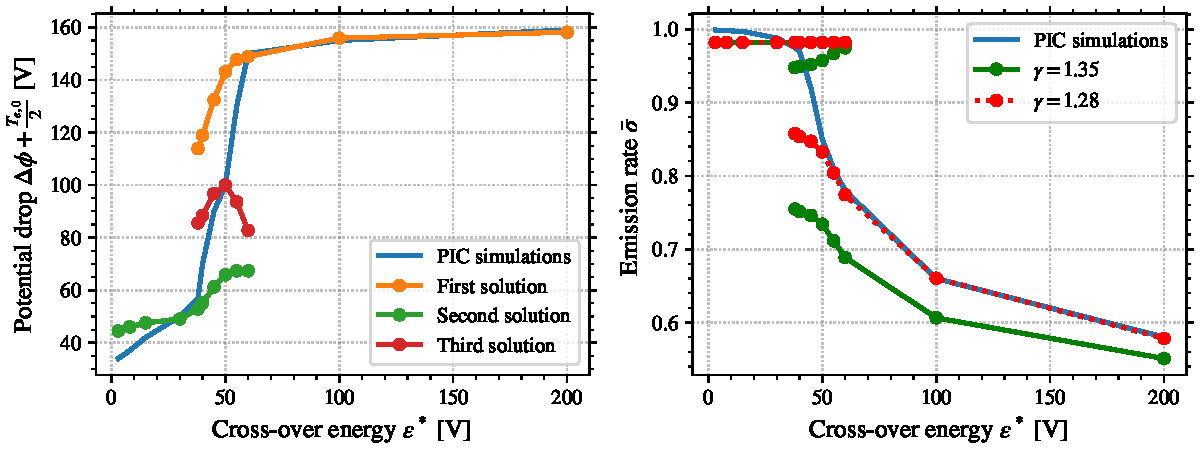
\includegraphics[width=\textwidth]{Poly_model_vs_pic}
      \caption{Comparison of the PIC simulations and the sheath model for the plasma potential drop from the center to the wall and the electron emission yield. }
      \label{fig-Poly_model_vs_pic}
    \end{figure}

    Concerning $\dphi$, we see that the sheath model combining the polytropic state law and the electron emission is in good agreement with the \ac{PIC} simulations.
    We see that the region where the three solutions coexist corresponds well with the regime {\bf II}.

    Concerning the emission rate $\rate$, we observe that the value $\gamma=1.35$ under estimates $\rate$ compared to the values of the \ac{PIC} simulations.
    On the other hand, $\gamma=1.28$ is in very good agreement.
    Interestingly, the saturation of the mean electron emission rate in the \ac{PIC} simulation is greater than the critical value $\ratecr$.
    
    %\inlinenote{ As $\rate$ is better with $\gamma=1.28$, we should use both values in \cref{eq-costseepoly}. However, this increases the complexity the equations and the model, and add 1 more free parameters (they would be 2 values for $\gamma$ now). I can say that only in the discussion maybe ? }
    
  \subsection{Sheath oscillations of regime {\bf II}} \label{subsec-pic_scheath_RSO}
  
    The regime {\bf II} is characterized by the presence of oscillations between two meta-stable regimes {\bf III} and {\bf I}, one with a low emissivity and the other with a high emissivity.
    \Cref{fig-long_time} shows the temporal evolution of the electron temperature and the plasma potential relative to the wall for $\crover=45\,\volt$.
    The electron temperature is computed over the whole electron population in the \ac{PIC} simulations.
    Both the radial temperature $\Te_{,R}$ and the total temperature $\Te$ are shown (see \cref{eq-3Te} for their definition).
    The plasma potential $\dphi$ shown is measured at the center of the radial direction of the simulation, averaged over the azimuthal direction.
    
    
    \begin{figure}[hbtp]
      \centering
      \begin{tabular}{c c}
        \subfigure{long_time_dphi}{a}{20,20} &
        \subfigure{long_time_Te}{b}{20,20} \\
      \end{tabular}
      \caption{Temporal evolution of ({\bf a}) the plasma potential $\dphi$ and ({\bf b}) the electron temperatures\string: $\Te_{,R}$ is the radial temperature, and $\Te$ is the total temperature.}
      \label{fig-long_time}
    \end{figure}

    
    We clearly see in \cref{fig-long_time} the quasi-periodic oscillations between the two states.
    We observe that the electron temperature is slightly anisotropic, with the radial temperature smaller than the axial temperature.
    This anisotropy observed was not taken into account in the sheath model.
    More precisely, the $\Te_{,R}$ is linked to the thermal flux of electron toward the wall, while the total temperature $\Te$ is used in the computation of the electron emission rate $\ratemaxw$.
    However, the degree of anisotropy is not very high, as it is of the order of 10\% when the sheath is not inverted.
    When the sheath is inverted, the anisotropy is of the order of 25\%, as the electron with a large radial energy are quickly absorbed.
    However in the \ac{SCL} regime, we suppose that the electron emission rate saturates at $\rate=\ratecr$, hence the impact of the total energy is less important with respect of the radial energy.
    Hence, we will compare the prediction using only the radial temperature $\Te_{,R}$ or the total, averaged, temperature $\Te$, but not the two of them together.
    
    \Cref{fig-dphi_te_PIc} shows the potential drop as a function of the radial electron temperature $\Te_R$ and the total electron temperature $\Te = (\Te_R + \Te_{\theta} + \Te_z)/3$ measured in the \ac{PIC} simulation (same case as \cref{fig-long_time}).
    Is also shown the theoretical solutions obtained with the model of \cref{sec-fluid_poly_see} using a constant polytropic index $\gamma=1.35$ and $\crover=45\,\volt$.
    
    \begin{figure}[hbtp]
      \centering
      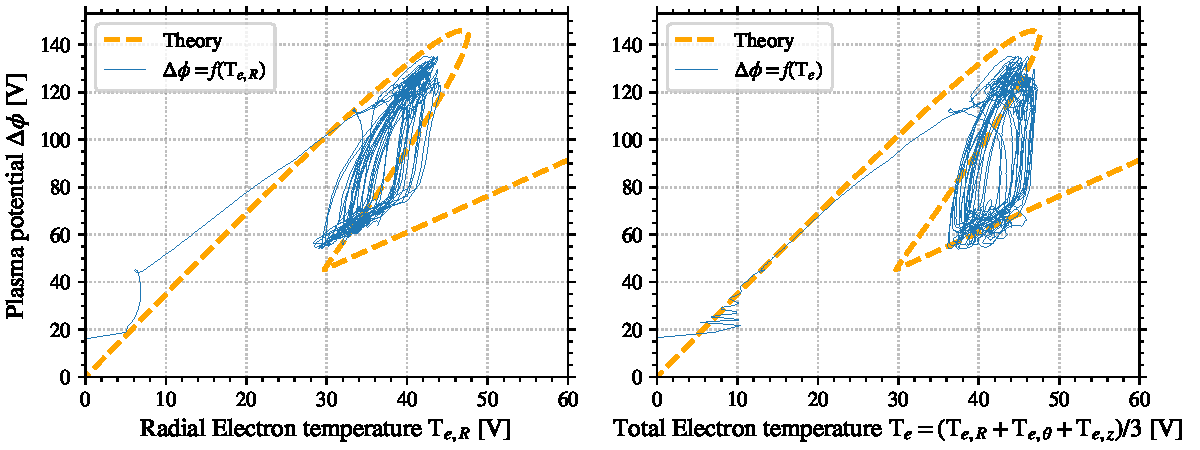
\includegraphics[width=\textwidth]{parametric_PIC_dphi_Te_bis}
      \caption{Plasma potential as a function of (left) the radial electron temperature and (right) the total electron temperature. The blue markers represent the \ac{PIC} results presented in \cref{fig-long_time}, and the orange dashed lines correspond to the theoretical values with $\gamma=1.35$.}
      \label{fig-dphi_te_PIc}
    \end{figure}
    
    We see in \cref{fig-dphi_te_PIc} that the sheath characteristics observed in the \ac{PIC}  simulations match relatively well the theoretically values.
    In particular, we see the cohabitation of the two solutions of $\dphi$ observed for the same electron temperature, which corresponds to the domain of electron temperature for which the sheath model also predicts multiple solutions.
    
    During the state corresponding to regime {\bf III} (high value of  $\dphi$), the \ac{PIC} values are too noisy to clearly determine if the sheath follows the first or the second branch of the solutions.
    On the other hand, we see relatively well the correspondance between the \ac{PIC} results and the theory for the regime {\bf I} (low value of $\dphi$).
    
    As discussed previously, the value of the polytropic index computed by propagating the \ac{EVDF}, is $\gamma=1.28$.
    \Cref{fig-dphi_te_PIc2} shows the same results as \cref{fig-dphi_te_PIc}, but  the theoretical values of $\dphi$ using $\gamma=1.28$ are overlaid.
    We see that using the value $\gamma=1.28$ does not change significantly the value of the solution, except for the maximum value of the electron temperature $\Te^1$ for the first branch of the solution, hence the domain of temperature where the three solutions coexist.
    In the case of $\gamma=1.28$, the \ac{PIC} simulation result agreement with the theory is worse than for $\gamma=1.35$.
    
    \begin{figure}[hbtp]
      \centering
      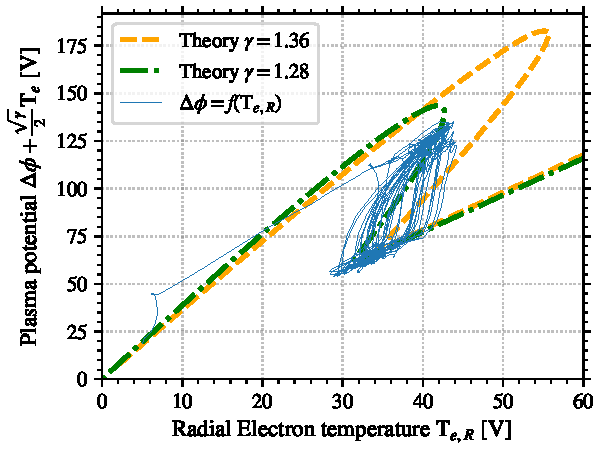
\includegraphics[width=\textwidth]{parametric_PIC_dphi_Te_two_gamma_bis}
      \caption{Similarly to \cref{fig-dphi_te_PIc}, Plasma potential as a function of (left) the radial electron temperature and (right) the total electron temperature. The blue markers represent the \ac{PIC} results presented in \cref{fig-long_time}, the orange dashed lines correspond to the theoretical values with $\gamma=1.35$, and the green dotted-dashed line is computed with $\gamma=1.28$.}
      \label{fig-dphi_te_PIc2}
    \end{figure}
    
    \paragraph{Stationary of the sheath \\}

    One has to note that the modified sheath model is stationary, while the oscillations observed are relatively fast.
    Indeed, the ion dynamic can be estimated to be
    \begin{equation} \label{eq-ti}
      \tau_i = \frac{2 \pi}{\opi} = 0.1 \,\micro\second.
    \end{equation}
    
    Another estimation of the ion time scale is the time needed by an ion to reach the sheath edge from the center of the discharge.
    Supposing a constant electric field $E_{\rm ps} = \frac{\Te}{L_R}$ in the pre-sheath, we have
    \begin{equation} \label{eq-tof}
      t_{\rm flight} = L_R \sqrt{\frac{m_i}{e \Te}} = 3.7 \,\micro\second.
    \end{equation}
    with $L_R=2\,\centi\meter$ and $\Te=40\,\volt$.
    The period of the sheath oscillations observed in \cref{fig-long_time} is approximately $T = 2\,\micro\second$, which is between $\tau_i$ and $t_{\rm flight}$.
    Hence, we can expect the ion dynamic to affect the plasma sheath characteristics during the sheath oscillations of the regime {\bf II}.
    
    \paragraph{Role of the ion mass \\}
    
    The sheath oscillations of regime {\bf II} have been observed in \citet{croes2017} with three different ion masses: xenon, krypton and argon.
    The results are shown in \cref{fig-RSO_altern}.
    We see that the period of the oscillations vary with the ion mass.
    More precisely, the period of oscillation decreases with the decrease of the ion mass.
    This observation confirm that the ions have a role in the dynamics of the oscillation.
    
    \begin{figure}[hbtp]
      \centering
      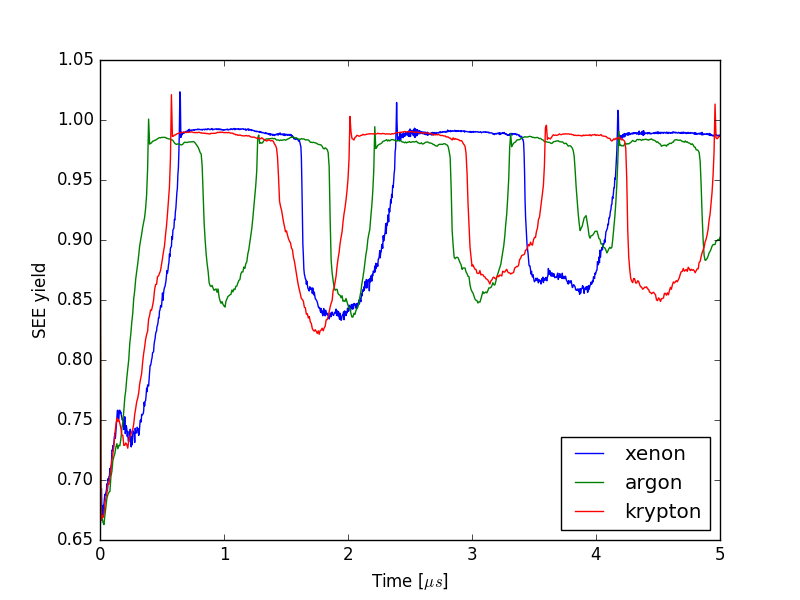
\includegraphics[width=\defaultwidth]{SEE_RSOs.png}
      \caption{Temporal evolution of the SEE rate $\rate$ measured in the PIC simulations for different gases (xenon, krypton, and argon), taken from \citet{croes2017}.}
      \label{fig-RSO_altern}
    \end{figure}
    
    
